%! Author = HP
%! Date = 21/07/2022

% Preamble
\documentclass{article}

% Packages
\usepackage[utf8]{inputenc}
\usepackage[spanish]{babel} % for lenguage
\usepackage{amsmath} % for equations
\usepackage{graphicx} % for images
\usepackage{float}  % for images
\usepackage{enumitem} %for listados
\usepackage{apacite}
\bibliographystyle{apacite}



\title{Practica-UNAL 12}
\author{Sergio Andrés Díaz Ariza \thanks{Este es un ensayo}}
\date{\today}

% Document
\begin{document}


\tableofcontents

\section{Energía Cinética} % Esto es una seccion
Sea $\vec{x}=(x_{1y},x_2,x_3)$ el vector de posición de una partícula de masa $m$,
    $\vec{v}=(dx_1/dt,dx_2/dt,dx_3/dt)$ y la acelaración $\vec{a}=(d^2x_1/dt,d^2x_2/dt,d^2x_3/dt)$.
    \\
    \textbf{La segunda Ley de Newton}\\
    \textit{La segunda Ley de Newton}\\
    \underline{\textbf{La segunda Ley de Newton}}\\
    \textbf{\textit{La Segunda Ley de Newton}}\\
    
    \section{Ecuaciones de Ambiente}
    \begin{equation}
        F_i = m*\frac{d^2x_i}{dt^2},\qquad i=1,2,3\dots \label{fuerza}
    \end{equation}

    Multiplicar por $i$ a la ecuación (\ref{fuerza})

    \begin{equation*}
        \frac{d}{dt}\left(\frac{m}{2}\sum_{i=1}^k\left(\frac{dx_i}{dt} \right)^2 \right|
    \end{equation*}
    \begin{equation*}
        \frac{d}{dt}\left|\frac{m}{2}\int_{i=1}^k \right)
    \end{equation*}

    De la funcion anterior \footnote{complicada la vaina}
    
    \section{Imagenes}
    Imagen del Telescopio James Webb 2022
    \begin{figure}[H]
        \centering
        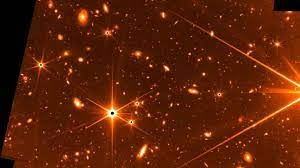
\includegraphics[height=5cm]{Images/James}
        \caption{James Webb Image}
        \label{img1}
    \end{figure}

    \section{Listado}
    Creamos un listado y ensayamos para Referenciar la imagen anterior~\ref{img1}
    \begin{itemize}[noitemsep]
        \item Laura
        \item Sergio
        \item Ismael
        \item \textit{Díaz}
    \end{itemize}

    Nueva Lista
    \begin{enumerate}[noitemsep,nolistsep]
        \item \textbf{Mayerly}
        \item Ariza
    \end{enumerate}

    \section{Tablas}
    \begin{table}[H]
        \centering
        \begin{tabular}{|c|c|}
            \hline
            Nombre & Apellido\\
            \hline
            Sergio & Díaz\\
            \hline
        \end{tabular}
        \caption{Nombres}
        \label{Tabla1}
    \end{table}

    \section{Bibliografia}
    Aqui citamos esa monda~\cite{mcfar}


    \bibliography{byblio}
    \bibliographystyle{apacite}




\end{document}

